\documentclass[a4paper,10pt]{article}
\usepackage{graphicx}
\usepackage{enumitem}
\usepackage{amsmath}
\usepackage{listings}
\usepackage[usenames,dvipsnames]{color}
\usepackage{bbm}
\usepackage{amsfonts}


%%%%%%%%%%%%%%%%%%%%%%%%%%%%%%%%%%%%%%%%%%%%%%%%%%%%%%%%%%%%%%%%%%%%%%%%%%%%%%%%%%%%%%%%%%%
% MATLAB code listing
%
% This is the color used for MATLAB comments below
\definecolor{MyDarkGreen}{rgb}{0.0,0.4,0.0}
 
% For faster processing, load Matlab syntax for listings
\lstloadlanguages{Matlab}%
\lstset{language=Matlab, % Use MATLAB
frame=single, % Single frame around code
basicstyle=\tiny\ttfamily, % Use small true type font
keywordstyle=[1]\color{Blue}\bfseries, % MATLAB functions bold and blue
keywordstyle=[2]\color{Purple}, % MATLAB function arguments purple
keywordstyle=[3]\color{Blue}\underbar, % User functions underlined and blue
identifierstyle=, % Nothing special about identifiers
% Comments small dark green courier
commentstyle=\usefont{T1}{pcr}{m}{sl}\color{MyDarkGreen}\small,
stringstyle=\color{Purple}, % Strings are purple
showstringspaces=false, % Don't put marks in string spaces
tabsize=5, % 5 spaces per tab
%
%%% Put standard MATLAB functions not included in the default
%%% language here
morekeywords={xlim,ylim,var,alpha,factorial,poissrnd,normpdf,normcdf},
%
%%% Put MATLAB function parameters here
morekeywords=[2]{on, off, interp},
%
%%% Put user defined functions here
morekeywords=[3]{FindESS, homework_example},
%
morecomment=[l][\color{Blue}]{...}, % Line continuation (...) like blue comment
numbers=left, % Line numbers on left
firstnumber=1, % Line numbers start with line 1
numberstyle=\tiny\color{Blue}, % Line numbers are blue
stepnumber=5 % Line numbers go in steps of 5
}

\usepackage{xspace}
\newcommand*{\eg}{e.g.\@\xspace}
\newcommand*{\ie}{i.e.\@\xspace}

\makeatletter
\newcommand*{\etc}{%
    \@ifnextchar{.}%
        {etc}%
        {etc.\@\xspace}%
}
\makeatother
%%%%%%%%%%%%%%%%%%%%%%%%%%%%%%%%%%%%%%%%%%%%%%%%%%%%%%%%%%%%%%%5

\newcommand\scalemath[2]{\scalebox{#1}{\mbox{\ensuremath{\displaystyle #2}}}}

%opening
\title{Auvitronics Design Department Procedure}
\author{Munzir Zafar}

\begin{document}

\maketitle

\begin{figure}[!ht]
\centering \frame{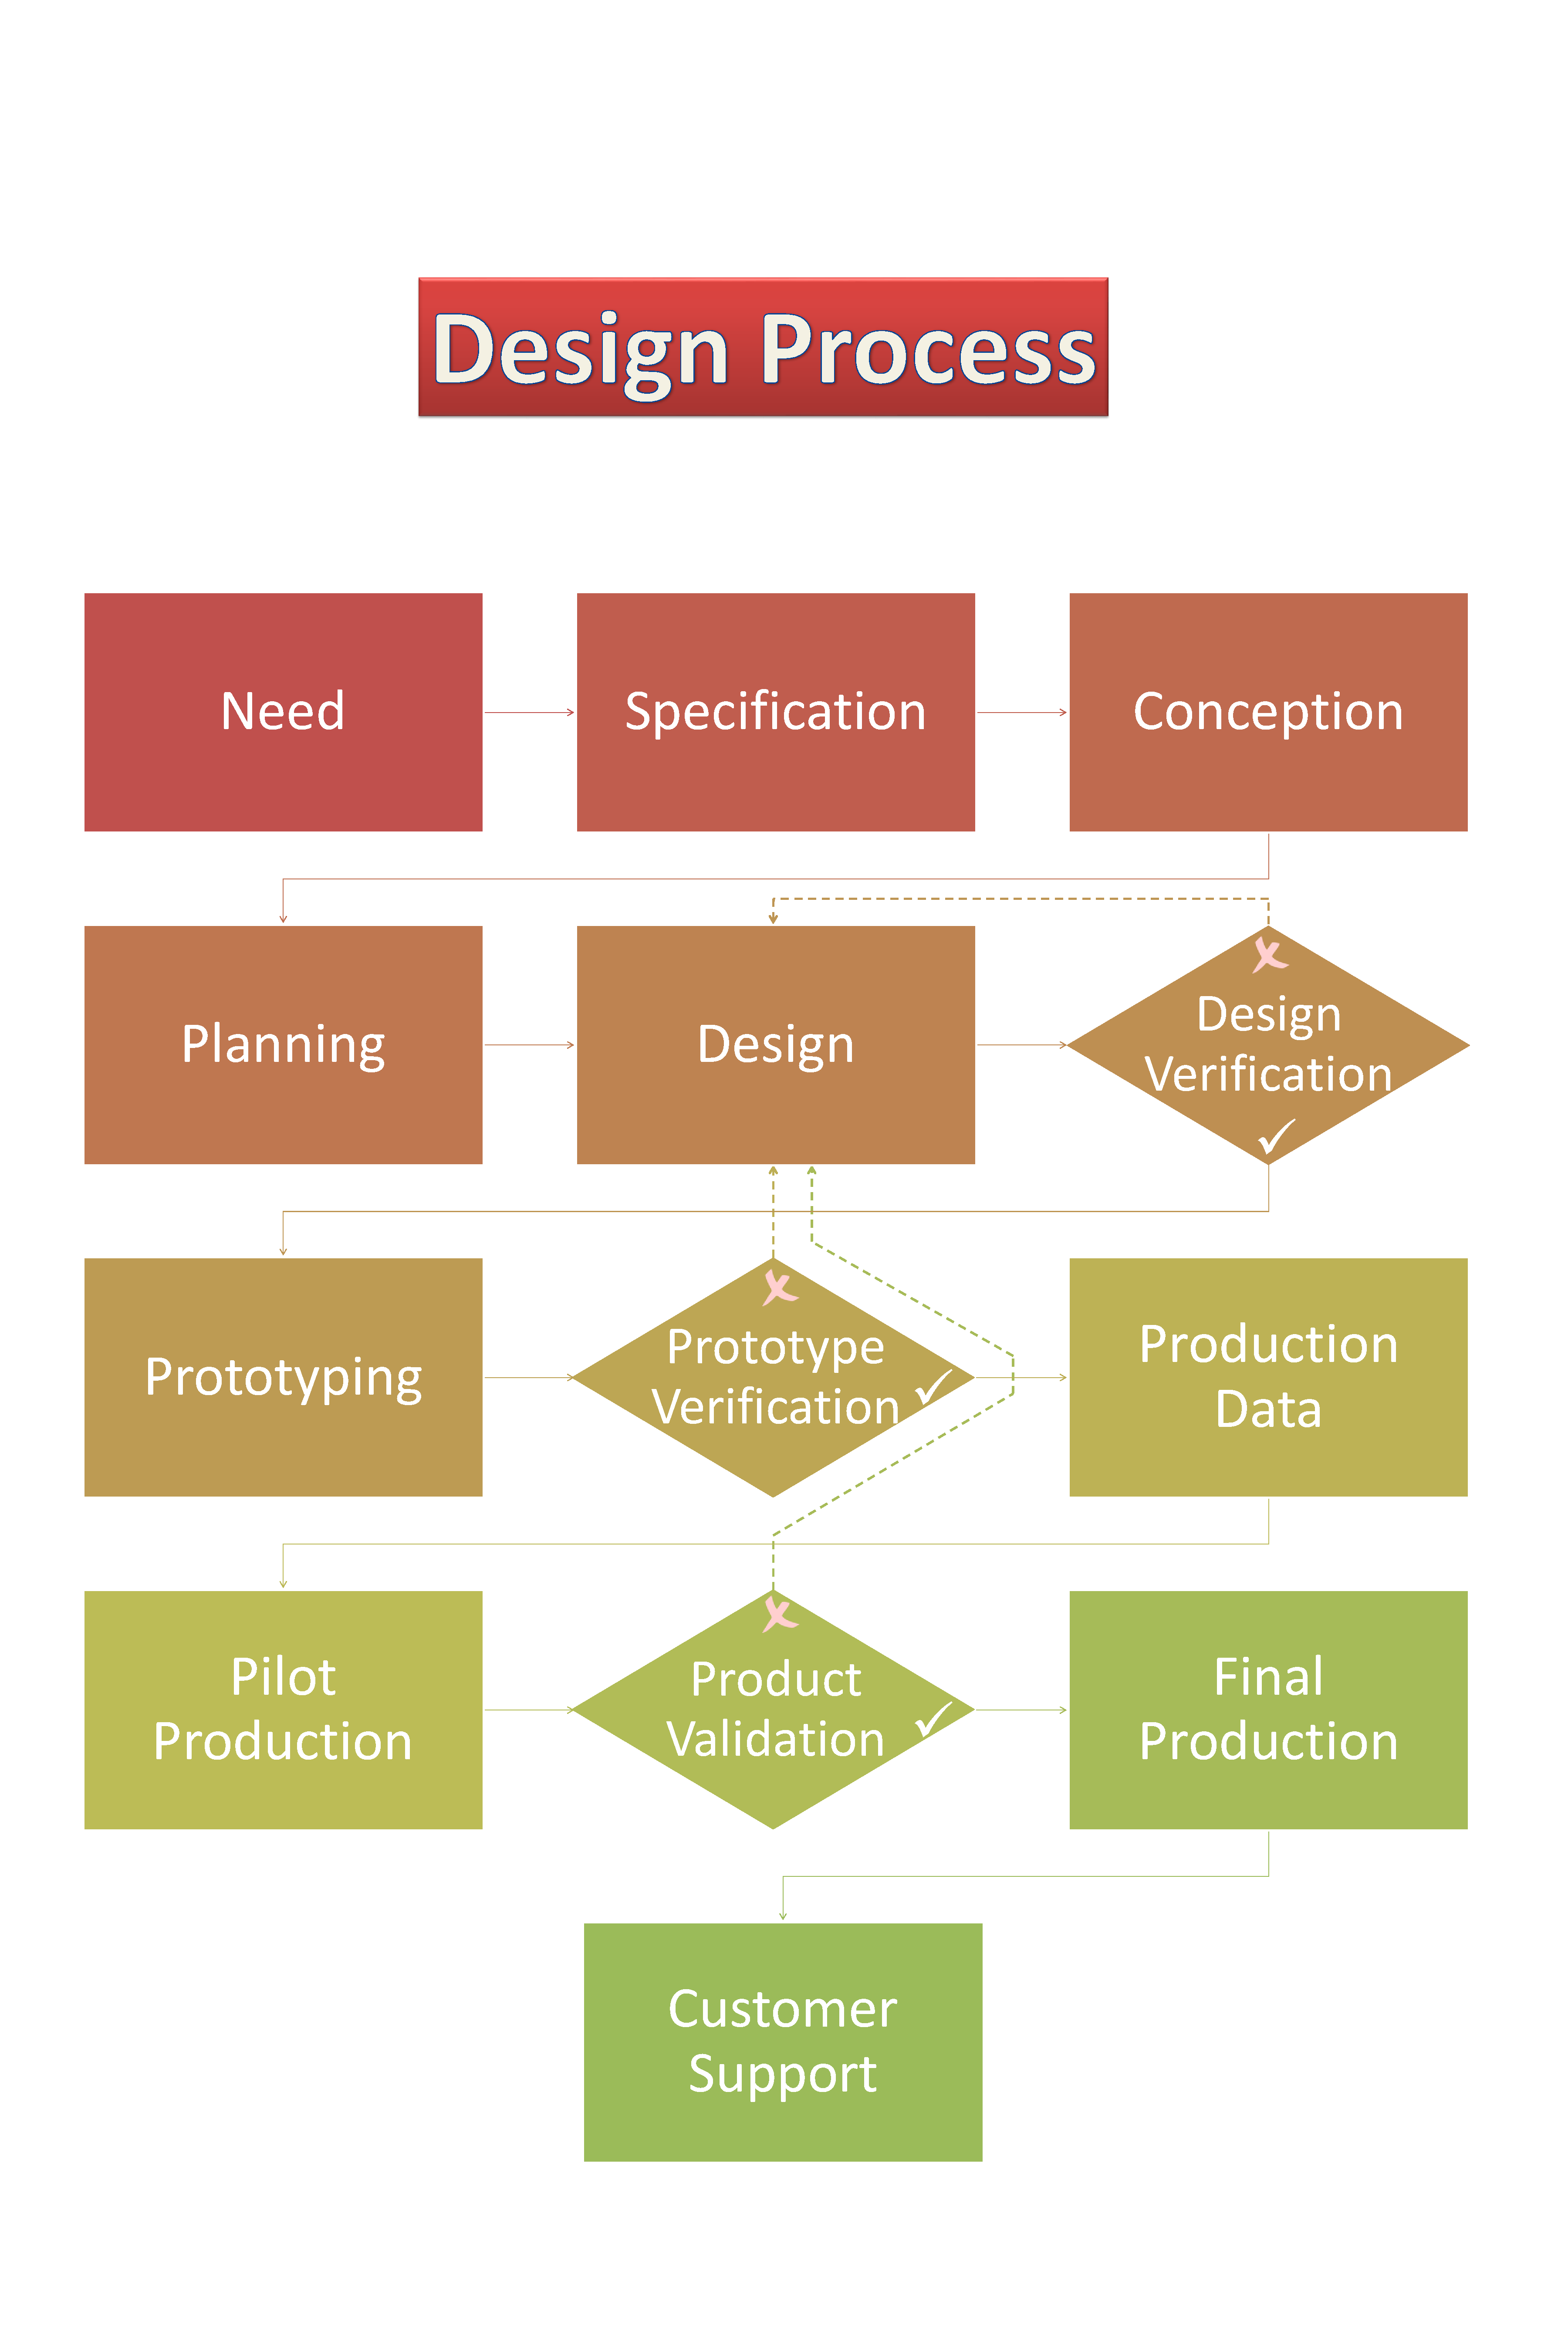
\includegraphics[width=0.8\columnwidth]{Figures/DesignProcess.pdf}}
\caption{Flowchart of the Design Process}
\label{fig:fig1} 
\end{figure}

\newpage
This document explains the design procedure to be used by the design department of Auvitronics. 

\section{Design Process}
Figure \ref{fig:fig1} shows a flowchart of the process that the department follows. In the following sections 
we briefly discuss each stage and the the deliverables expected at the end of each stage.

\subsection{Need}
Any new project is initiated with the proposal or approval of a project idea by the upper management. This 
idea will be based on certain motivations driven by any one of the following:
\begin{itemize}
 \item Customer needs
 \item Anticipation of a potential market
 \item Manufacturing process improvement or automation needs within the company
\end{itemize}
The \emph{Statement of Need} will be written down establishing the needs and goals for the project. This will
be approved by the management so that exact needs are well-established among all stake-holders of the project.

\subsection{Specifications}
The needs or goals established in the earlier step have to be translated in this stage into technical specifications
that will serve as design goals for the technical team delivering the project. These specifications may include design specifications,
testing specifications, certification or compliance with standards, how the product will be maintained throughout its life-time.

The \emph{Specifications} document may have the following sample headings:
\begin{itemize}
 \item Introduction
 \item Environment
 \item Performance
 \item Physical Size and Weight
 \item Power
 \item Life
 \item Reliability
 \item Cost
 \item Manufacturing Process
 \item Maintenance
\end{itemize}

\subsection{Conception}
In this stage, the conceptual design of the product will be finalized. All possible design solutions will be 
considered. The pros and cons of each design will be weighed. Uncertainties in the decision-making process
may require proof of certain new concepts that are being considered, and may lead to quick research 
or development sub-projects aimed at proving the new concepts. Based on the all available information regarding
costs, time, resources and the like required in each alternative solution, one will be selected that minimizes the costs and maximizes the utility for the end-user. 
Other considerations may include manufacturability, ease of testing, maintainability, scaleability,
service/support costs and running costs of the designs being considered. 
This \emph{Conception} document will be delivered by system-designers that may include several inputs from the 
upper management as well as the design engineers, production team, manufactureres, suppliers etc. And the document should explain clearly
the decision-making process used to choose one design solution among many.

\subsection{Planning}
In this stage a \emph{Project Plan} will be initiated, where:
\begin{enumerate}
 \item Components of the system will be identified
 \item It will be identified which components will be designed in-house and which will be purchased off the shelf
 \item For off-the-shelf purchases, the suppliers will be finalized 
 \item For in-house production and design responibilities and timelines will be assigned
 \item Testing procedures for in-house designs will be determined and planned with responsibilities and timelines assigned
 \item Overall project timeline will be determined, clearly stating---for each designed component, sub-assembly, full assembly and testing equipment built in-house---the stages of:
 design, design-verification, prototyping, prototype-verfication, pilot production and product validation. Responsibilities and timelines for each will be allocated.
 \item Reporting requirements will be determined. These may include mechanism for reporting design progress to upper management, 
 mechanism for reviewing the project plan on a regular basis \etc
 \item Documentation requirements will be determined and assigend. These may include: Designing of brochures, user guides, installation
 guides etc.
\end{enumerate}

The next six stages: Design, design-verification, prototyping, prototype-verfication, production data and product validation will be 
followed separately for each designed component, sub-assembly, full assembly and testing equipment built in-house.

\subsection{Design}
In this stage, the following documents will be delivered, as applicable:
\begin{itemize}
 \item Engineering drawings, assembly drawings and material specifications
 \item Schematic diagrams and wiring diagrams
 \item Algorithms, codes and software documentation that goes with it
 \item Documents providing rationale for each design decisions not immediately apparent in the supplied drawings and schematics
 \item Documents detailing production and maintenance processes for the designed part
\end{itemize}

\subsection{Design Verification}
Mathematical analysis or computer simulations of the designs will be carried out, if possible, to prove mathematically that the suggested design meets the 
design requirements. Upon failure to meet the requirements, design will be reviewed and revised. \emph{Design Review} document will
state the results of verification and comments on the reasons of failure, if any.

\subsection{Prototype}
Initial material list to be purchased will be prepared called the \emph{Prototype Material List} and an initial production procedure
for the prototype will be prepared called \emph{Prototype Production Procedure}. Then, preferably with the help/involvement of the production team, models of the design will be developed, such as circuit boards (vero-boards) for electronic circuits, or cheaply constructed assemblies for mechanical parts etc. New production equipment or training should be identified at this stage.

\subsection{Prototype Verification}
The prototypes will be verified according to the testing procedures. Upon failure to meet the requirements, design will be reviewed and revised.
The \emph{Prototype Review} document will state the results of the verification and comments on the reasons of failure, if any.

\subsection{Production Data}
Necessary data that needs to be prepared for production of the finalized design will be delivered. This may include PCB layouts, mold data and the like.


\subsection{Pilot Production}
Upon verification of the prototype of the full assembly, a \emph{Final Material List} and \emph{Final Production Procedure} 
will be handed over to the production team which will be required to produce the product in small quantity with support from the design department,
if any. The in-house testing of each produced product should be carried out as part of the quality assurance procedure by 
the production team itself. Such testing procedures should be part of the \emph{Final Production Procedure} delivered by the design team.

\subsection{Product Validation}
The final product will be delivered to the customer, and verified according to agreed testing specifications and customer sign-off will be obtained as a
sign of customer satisfaction. 

\subsection{Final Production}
Large-scale prodcution or as-per-requirement will now be setup as a final stage of complete handover of the project from the design team to the
production team.

\subsection{Customer Support}
User guides, maintenance guides, repair guides, design improvements upon feedback from the customer or the production team or the service/repair teams
will be the responsibility of the design department for the remaining life of the product or till the time the product is stable.

\section{Deliverables}

Based on the above description, following is the list of documents to be delivered for any project to be carried out by the department:
\begin{enumerate}
 \item Statement of Need
 \item Requirements Specifications
 \item System Conception
 \item Project Plan
 \item Design documents
  \begin{enumerate}
    \item Drawings of parts, assemblies with material specifications
    \item Schematics and Wiring Diagrams
    \item Codes, software
    \item Documentation stating rationale for each design decision
  \end{enumerate}
 \item Design Review
 \item Prototype material list
 \item Prototype production procedure
 \item Prototype review
 \item Production data (PCB data, mold data, and the like)
 \item Final material list
 \item Final production procedure
 \item User guide
 \item Maintenance guide
\end{enumerate}


\end{document}

